\section{Introduction} \label{sec:introduction}

The BDZ algorithm was designed by Fabiano C. Botelho, Djamal Belazzougui, Rasmus Pagh and Nivio Ziviani.
It is a simple, efficient, near-optimal space and practical
algorithm to generate a family $\cal F$ of PHFs and MPHFs.
It is also referred to as BPZ algorithm because the work presented
by Botelho, Pagh and Ziviani in \cite{bpz07}.
In the Botelho's PhD. dissertation \cite{b08} it is also referred to as RAM algorithm
because it is more suitable for key sets that can be handled in internal memory.

The BDZ algorithm uses $r$-uniform random hypergraphs
given by function values of $r$
uniform random hash functions on the input key set $S$ for generating PHFs and MPHFs that
require $O(n)$ bits to be stored.
A hypergraph is the generalization of a standard undirected
graph where each edge connects $r\geq 2$ vertices.
This idea is not new, see e.g. \cite{mwhc96},
but we have proceed differently to achieve
a space usage of $O(n)$ bits rather than $O(n\log n)$ bits.
Evaluation time for all schemes considered is constant. 
For $r=3$ we obtain a space usage of approximately $2.6n$ bits for 
an MPHF. More compact, and even simpler, representations can be
achieved for larger $m$. For example, for $m=1.23n$ we can get a
space usage of $1.95n$ bits.

Our best MPHF space upper bound is within a
factor of 2 from the information theoretical lower bound of approximately
$1.4427n$ bits. We have shown that the BDZ algorithm is far more
practical than previous methods with proven space complexity, both
because of its simplicity, and because the constant factor of the
space complexity is more than 6 times lower than its closest
competitor, for plausible problem sizes. We verify the practicality
experimentally, using slightly more space than in the mentioned
theoretical bounds.

\section{The Algorithm}

The BDZ algorithm is a three-step algorithm that generates PHFs and MPHFs based on
random $r$-partite hypergraphs.
This is an approach that provides a much tighter analysis and is
much more simple than the one presented in
\cite{ckrt04}, where it was implicit how to construct 
similar PHFs.
The fastest and most compact functions
are generated when $r=3$.
In this case a PHF can be stored in
approximately $1.95$ bits per key and 
an MPHF in approximately 
$2.62$ bits per key.

Figure~\ref{fig:overview} gives an overview of the algorithm for $r=3$, 
taking as input a key set $S \subseteq U$ containing three English words, i.e.,  $S=\{\mathrm{who},\mathrm{band},\mathrm{the}\}$.
% which are nicely hashed to the name of a rock band ``the who band''. 
The edge-oriented data structure proposed in~\cite{e87} is used 
to represent hypergraphs, where each edge is explicitly represented
as an array of $r$ vertices and, for each vertex $v$,
there is a list of edges that are incident on $v$.

The {\em Mapping Step} in Figure~\ref{fig:overview}(a) carries out two 
important tasks:
\begin{enumerate}
\item 
It assumes that it is possible to find three uniform 
hash functions, $h_0$, $h_1$ and $h_2$, with ranges $\{0,1\}$, $\{2,3\}$ and $\{4,5\}$, respectively.
These functions build an one-to-one mapping of the key set $S$ to the edge set $E$
of a random acyclic  
$3$-partite hypergraph $G=(V,E)$, where $|V|=m=6$ and $|E|=n=3$.
In \cite{b08,bpz07} it is shown that
it is possible to obtain such a hypergraph with probability tending to $1$ as $n$
tends to infinity
whenever $m=cn$ and $c \ge 1.23$. The value of $c$ that minimizes the hypergraph size 
(and thereby the amount of bits to represent the resulting functions) is $c \approx 1.23$.
To illustrate the mapping, 
key ``who'' is mapped to edge $\{h_0(\text{``who''}),h_1(\text{``who''}),h_2(\text{``who''})\}=\{1,3,5\}$, 
key ``band'' is mapped to edge $\{h_0(\text{``band''}),h_1(\text{``band''}),h_2(\text{``band''})\}=\{1,2,4\}$, and 
key ``the'' is mapped to edge $\{h_0(\text{``the''}),h_1(\text{``the''}),h_2(\text{``the''})\}=\{0,2,5\}$. 
\item
It tests whether the resulting random $3$-partite hypergraph contains cycles
by iteratively deleting edges connecting vertices of degree 1.
The deleted edges are stored in the order of deletion in a list $\cal L$
to be used in the assigning step. 
The first deleted edge in Figure~\ref{fig:overview}(a)
was $\{1,2,4\}$, the second one was $\{1,3,5\}$ and 
the third one was $\{0,2,5\}$.
% the last one was $\{0,2,5\}$.
If it ends with an empty graph, then the test succeeds,
otherwise it fails. 
\end{enumerate}


\begin{figure}
\begin{center}
\scalebox{0.9}{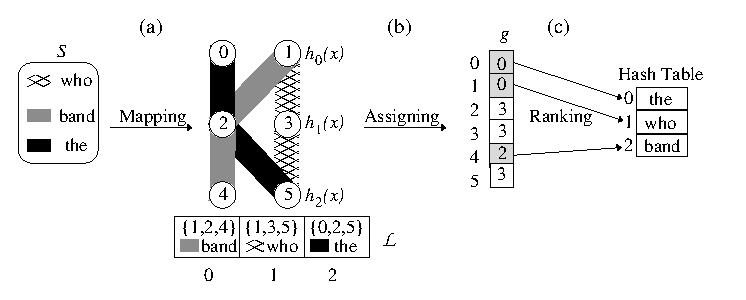
\epsfig{file=figs/overviewinternal3g.eps}}
\end{center}
\caption{(a) The mapping step generates a random acyclic $3$-partite hypergraph with $m=6$ vertices and $n=3$ edges
and a list $\cal L$ of edges obtained when we test whether the hypergraph is acyclic.
(b) The assigning step builds an array $g:[0,5] \to [0,3]$ to uniquely
assign an edge to a vertex. (c) The ranking step builds the data structure used to 
compute function $\mathit{rank}: [0,5] \to [0,2]$ in $O(1)$ time.~~~~}
\label{fig:overview}
\end{figure}



We now show how to use the Jenkins hash functions \cite{j97}
to implement the three hash functions $h_i: S \to V_i$, $0\le i \le 2$, which are used to build a random $3$-partite hypergraph
$G=(V,E)$,
where $V= V_0 \cup V_1 \cup V_2$ and $|V_i| = \eta = \lceil \frac{m}{3} \rceil$.
Let $h':S \to \{0,1\}^\gamma$ be a Jenkins hash function
for $\gamma = 3 \times w$, where
$w = 32 \text{ or } 64$ for
32-bit and 64-bit architectures, respectively. 
Let $H'$ be an array of 3 $w$-bit values.
The Jenkins hash function
allow us to compute in parallel the three entries in $H'$
and thereby the three hash functions $h_i$, as follows:
% Thus we can compute the three hash functions $h_i$ 
% as follows:
\begin{eqnarray}
 H' &=& h'(x) \nonumber \\
 h_0(x) &=& H'[0] \bmod \eta \nonumber \\
 h_1(x) &=& H'[1] \bmod \eta + \eta \nonumber \\
 h_2(x) &=& H'[2] \bmod \eta + 2\eta
\end{eqnarray}

The {\em Assigning Step} in Figure~\ref{fig:overview}(b) outputs 
a PHF that maps the key set $S$ into the range $[0,m-1]$ and is represented by
an array $g$ storing values from the range $[0,3]$.
The array $g$ allows to select one out of the $3$
vertices of a given edge, which is associated with a 
key $k$.
A vertex for a key $k$ is given
by either $h_0(k)$, $h_1(k)$ or $h_2(k)$.
The function $h_i(k)$ 
to be used for $k$ is chosen by calculating $i = (g[h_0(k)] + g[h_1(k)] + g[h_2(k)]) \bmod 3$.
For instance,
the values 1 and 4 represent the keys ``who'' and ``band'' 
because $i = (g[1] + g[3] + g[5]) \bmod 3 = 0$ and $h_0(\text{``who''}) = 1$,
and $i = (g[1] + g[2] + g[4]) \bmod 3 = 2$ and $h_2(\text{``band''}) = 4$, respectively.
% Likewise, the value 4 represents the key  
% because $(g[1] + g[2] + g[4]) \bmod 3 = 2$ and $h_2(\text{``band''}) = 4$, and so on. 
The assigning step firstly initializes $g[i]=3$
to mark every vertex as unassigned  
% (i.e., each vertex is unassigned) 
and
$\mathit{Visited}[i]=\mathit{false}$, $0\leq i \leq m-1$.
Let $\mathit{Visited}$ be a boolean vector of size $m$
to indicate whether a vertex has been visited.
Then, for each edge $e \in \cal L$ from tail to head, 
it looks for the first
vertex $u$ belonging to $e$ not yet visited. 
This is a sufficient condition for success \cite{b08,bpz07,mwhc96}.
Let $j$, $0 \leq j \leq 2$, be the index of $u$ in $e$. 
Then, it assigns $g[u]=(j-\sum_{v \in e \wedge \mathit{Visited}[v] = true} g[v]) \bmod 3$. 
Whenever it passes through a vertex $u$ from $e$, 
if $u$ has not yet been visited,
it sets $\mathit{Visited}[u] = true$.
% The value $g[i]=3$ is used to represent unassigned vertices.

If we stop the BDZ algorithm in the assigning step
we obtain a PHF with range $[0,m-1]$.
The PHF has the following form:
$phf(x) = h_{i(x)}(x)$, where $x\in S$ and $i(x) = (g[h_0(x)] + g[h_1(x)] + g[h_2(x)]) \bmod 3$.
In this case we do not need information for ranking and
can set $g[i] = 0$ whenever $g[i]$ is equal to 3, where $0 \le i \le m-1$.
Therefore, the range of the values stored in $g$ is narrowed 
from $[0,3]$ to $[0,2]$. By using arithmetic coding as block of 
values (see \cite{b08,bpz07} for details),
or any compression technique that allows to perform 
random access in constant time to an array of compressed values \cite{fn07,gn06,sg06},
we can store the resulting PHFs in $m\log 3  = c n\log 3$ bits, 
where $c \ge 1.23$. For $c = 1.23$, the space requirement is $1.95n$ bits.


The {\em Ranking Step} in Figure~\ref{fig:overview}(c)
outputs a data structure 
that permits to narrow the range of a PHF generated in the
assigning step from $[0,m-1]$ to $[0,n-1]$ and thereby 
an MPHF is produced.
The data structure allows to compute in constant time 
a function $\mathit{rank}\!\!:[0,m-1]\to [0,n-1]$ 
that counts the number of assigned positions 
before a given position $v$ in $g$.
For instance, $\mathit{rank}(4) = 2$ because 
the positions $0$ and $1$ are assigned 
since $g[0] \text{ and } g[1] \not = 3$.
% and they come before position 4 in $g$.

For the implementation of the ranking step 
we have borrowed 
a simple and efficient implementation from
\cite{dict-jour}. 
It requires $\epsilon \, m$ additional bits of space, where $0 < \epsilon < 1$,
and is obtained by storing explicitly the
$\mathit{rank}$ of every $k$th index in a rankTable, where $k
=\lfloor\log(m)/\epsilon\rfloor$.
The larger is $k$ the more compact is the resulting MPHF.
Therefore, the users can tradeoff space for evaluation time
by setting $k$ appropriately in the implementation. 
% In the implementation we let 
% $k$ to be set by the users so that they can trade off
% space for evaluation time and vice-versa. 
We only allow values for $k$
that are power of two (i.e., $k=2^{b_k}$ for some constant $b_k$) in order to replace the expensive
division and modulo operations by 
bit-shift and bitwise ``and'' operations, respectively.
We have used $k=256$ 
in the experiments
for generating more succinct MPHFs.
We remark that it is still possible to obtain a more compact data structure by 
using the results presented in \cite{os07,rrr02}, but at the cost of a much more
complex implementation.

We need to use an additional lookup table $T_r$
to guarantee the constant evaluation time of $\mathit{rank}(u)$.
Let us illustrate how $\mathit{rank}(u)$ is computed
using both the rankTable and the lookup table $T_r$.
We first look up 
the rank of the largest precomputed index
$v\leq u$ in the rankTable, 
and use $T_r$ to count the number of assigned vertices from position
$v$ to $u-1$.
The lookup table $T_r$ allows us to count in constant time
the number of assigned vertices in $\flat=\epsilon \log m$ bits,
where $0 < \epsilon  < 1$. Thus the actual evaluation time is $O(1/\epsilon)$.
For simplicity and
without loss of generality we let $\flat$ be a multiple of the number of
bits $\beta$ used to encode each entry of $g$.
As the values in $g$ come from the range $[0,3]$,
then $\beta=2$ bits and we have tried $\flat = 8 \text{ and } 16$.
We would expect that $\flat = 16$ should provide 
a faster evaluation time because we would need to carry out fewer lookups
in $T_r$. But, for both values of $\flat$ the lookup table $T_r$ fits entirely in 
the CPU cache and we did not realize any significant difference in 
the evaluation times. Therefore we settle for $\flat=8$.
We remark that each $r \ge 2$ requires 
a different lookup table $T_r$ that can be generated a priori.


% To do this in $O(1/\epsilon)$  time
% we use a lookup table $T_r$ that allows us to count
% the number of assigned vertices in $\flat=\epsilon \log m$ bits
% in constant time for any $0 < \epsilon  < 1$. 



% In general the PHFs or MPHFs are constructed based on random acyclic $r$-partite hypergraphs $G_r=(V,E)$, 
% where $V= V_0 \cup V_1 \cup \dots \cup V_{r-1}$ and $|V_i| = \eta = \lceil \frac{m}{r} \rceil$, where $0\leq i < r$.
% The most efficient and compact functions are generated  
% when $r=3$ and $m=1.23n$. The value $1.23n$ is required to generate a
% random acyclic $3$-partite hypergraph with high probability\footnote{Throughout this paper 
% we write ``with high probability'' to mean with probability
% $1 - n^{-\delta}$ for $\delta > 0$.}~\cite{b08,bpz07}.


% the family of linear transformations
% presented in \cite{admp99}. A still faster option is the Jenkins function
% proposed in \cite{j97}, which was used for all methods considered in this paper.

The resulting 
MPHFs have the following form:
$h(x) = \mathit{rank}(\mathit{phf}(x))$.
Then, we cannot get rid of
the raking information by replacing the values 3 by 0 in the entries of $g$.
% The array 
% $g$ is now representing a function $g:V\to \{0,1,2,3\}$
% and $\mathit{rank}: V \to [0,n-1]$ is 
% now the cardinality of 
% $\{ u\in V \;\mid\; u<v \wedge g[u] \not = 3\}$.
% Notice that a vertex $u$ is assigned if $g[u] \neq 3$.
In this case each entry in the array $g$ is encoded 
with $2$ bits and we need $\epsilon m$ additional bits to compute function
$\mathit{rank}$ in constant time. Then, the total space to store 
the resulting functions is $(2 + \epsilon)m = (2 + \epsilon)cn$ bits.
By using $c = 1.23$ and $\epsilon = 0.125$
we have obtained MPHFs that require approximately $2.62$ bits per key to be stored.

% Figure~\ref{prog:ram} presents a pseudo code for 
% the BDZ algorithm, showing how to implement the mapping,
% assigning, and ranking steps. Next, it shows how to evaluate the PHF and the MPHF.
% The MPHF algorithm uses a lookup table, which is also shown in the figure.
% 
% \begin{figure}
% \begin{center}
% \vspace{-10mm}
% \begin{lstlisting}[multicols=2]
% @{\bf BDZ Algorithm}\\[1mm]@
% @{\bf Input:}  key set $S$, a constant $c \ge 1.23$, a constant $b_k$ 
% and a family of ``good'' hash functions $\cal H$.\\[1mm]@
% @{\bf Output:} an array $g$ with $m = \lceil cn \rceil$ 2-bit entries, and a rankTable with $(m >\!> b_k + 1)$ $\delta$-bit entries, where $\delta = 32 \text{ or } 64$ depending on the architecture. The operator $>\!>$ denotes the right shift of bits.\\[2mm]@ 
% void @BDZ@ (@$S$@, @$\cal H$@, @$c$@, @$b_k$@, @$g$@, @rankTable@)@\\[2mm]@ 
%    // Mapping step
%    do 
%      @$G.E = \emptyset$@;
%      select @$h'$@ at random from @$\cal H$@;
%      for @{\bf each}@ @$x \in S$@ do
%        @$H'$ = $h'(x)$@;
%        @$e$@ = @$\{h_0(x), h_1(x), h_2(x)\}$@;
%        addEdge (@$G$@, @$e$@);
%        @$\cal L$@ = isAcyclic(@$G$@);
%    while (@$G.E$@ is not empty);
% 
%    // Assigning step
%    for (@$u = 0$@; @$u < m$@; @$u$++@) 
%      Visited[@$u$@] = @{\bf false}@;
%      @$g[u]$@ = @$3$@;
%    for (i = @$|{\cal L}|-1$@; i @$\ge 0$@; i@$--$@)
%      @$e$@ = @$\cal L$@[i]; 
%      sum = 0;
%      for (@$v$@ = 2; @$v \ge 0$@; @$v$@@$--$@)
%        if (not Visited[@$e[v]$@])
%          Visited[@$e[v]$@] = @{\bf true}@;
%          @$u$@ = @$e[v]$@;
%          @$j$@ = @$v$@;
%        else sum += @$g[e[v]]$@;
%      @g[u]@ = @$(j - \mathrm{sum}) \bmod 3$@;
% 
%    // Ranking step
%    sum = 0;
%    kmask = @$(2^{b_k}-1)$@;
%    for (i = 0; i < @$|g|$@; i++)
%      if((i & kmask) @==@ 0) 
%        rankTable[i @$>\!> b_k$@] = sum;
%      if(@$g$@[i] @$\not = 3$@) sum++;
% 
% @{\bf PHF Algorithm}\\[1mm]@
% @{\bf Input:}  a key $x \in S$, an array $g$ with $m = \lceil cn \rceil$ 2-bit entries, where $c \ge 1.23$, and the ``good'' hash functions $h'$ selected by the BDZ algorithm.\\[1mm]@
% @{\bf Output:} the perfect hash function value for the key $x \in S$.\\[2mm]@
% int phf (@$x$@, @$g$@, @$h'$@)
%    @$H'$@ = @$h'(x)$@;
%    @$e$@ = @$\{h_0(x), h_1(x), h_2(x)\}$@;
%    @$v$@ = @$(g[e[0]] + g[e[1]] + g[e[2]]) \bmod 3$@;
%    return @$e[v]$@;
% 
% @{\bf Algorithm to Generate the Lookup Table}\\[1mm]@
% @{\bf Input:}  none\\[1mm]@
% @{\bf Output:} the lookup table @$T_r$@ to be used by the mphf function. It counts the number of assigned 
% vertices in a single byte. As each entry in the array $g$ is encoded by 2 bits, then a single byte can store at most four 2-bit values. LS($i'$,2) stands for the value of the 2 least significant bits of $i'$.\\[2mm]@
% void genLookupTable (@$T_r$@)
%    for (i = 0; i < 256; i++)
%      sum = 0; 
%      @$i'$@ = i;
%      for (j = 0; j < 4; j++)
%        if(@$\text{LS}(i',2) \not = 3$@) sum++;
%        @$i'$@ = @$i' >\!> 2$@;
%      @$T_r[i]$@ = sum;
% 
% @{\bf MPHF Algorithm}\\[1mm]@
% @{\bf Input:}  a key $x \in S$, an array $g$ with $m = \lceil cn \rceil$ 2-bit entries, where $c \ge 1.23$, the chosen ``good'' hash functions $h'$, a constant $b_k$ that makes $k=2^{b_k}$, the lookup table $T_r$ that counts the number of assigned vertices in a single byte, and a rankTable with $(m >\!> b_k + 1)$ $\delta$-bit entries, where $\delta = 32 \text{ or } 64$ depending on the architecture. The notation $g[i \to j]$ represents the values stored in the entries from $g[i]$ to $g[j]$ for $i\leq j$.\\[1mm]@
% @{\bf Output:} the minimal perfect hash function value for the key $x \in S$.\\[2mm]@
% int mphf (@$x$@, @$g$@, @$h'$@, @$b_k$@, @$T_r$@, @rankTable@)
%    @$u$@ = phf(@$x$@, @$g$@, @$h'$@);
%    j = @$u >\!> b_k$@; // @j@ = @$u$@/k
%    rank = rankTable[j];
%    i = j @$<\!< b_k$@; // @i@ = @j*k@
%    for(j = i + 4; j < u; i = j, j += 4)
%       rank += @$T_r[g[$@i @$\to$@ j@$]]$@;
%    for(j = j - 4; j < u; j ++)
%       if(@$g$@[j] @$\not =$@ 3) rank ++ ;
%    return rank;
% \end{lstlisting}
% \end{center}
% \vspace{-6mm}
% \caption{The BDZ algorithm and the resulting PHFs and MPHFs.}
% \label{prog:ram}
% \vspace{-7mm}
% \end{figure}

$\eta$ ~~
$\epsilon$ ~~
$\varepsilon$